\section{Résolution d'équations différentielles ordinaires}\label{sec:sec1}
Les algorithmes de résolution présentés ici utilisent tous des méthodes avec un pas de discrétisation, de la forme
$y_{n+1}=y_n+h_n \times \phi (y_n,t_n,h_n)$. En pratique, on cherche à mettre l'équation différentielle sous la forme d'un problème de Cauchy.
Cela fait intervenir une fonction $f$ et une fonction $y$ ainsi que sa dérivée, ainsi qu'un vecteur de conditions initiales $y_0$.
On a alors $y'(t)=f(y(t),t)$, et $y(t_0)=y_0$.

\subsection{Méthodes de résolution}
Nous avons implémenté les méthodes de résolution d’Euler, du point-milieu, de Heun et de Runge-Kutta.
Ces méthodes se basent sur des équations donnant $y_{n+1}$ en fonction de $y_n$, $h_n$ et $t_n$.

Une fonction a donc été réalisée pour chacune de ces méthodes, et permet d'effectuer un unique pas de temps.
Les fonctions détaillées dans la suite réutiliseront ces fonctions, en effectuant un nombre d'itérations défini, selon la méthode choisie.

Nous avons implémenté \texttt{meth\_n\_step} qui calcule un nombre $N$ d'étapes avec un pas constant $h$,
puis \texttt{meth\_epsilon} qui calcule une solution approchée avec un paramètre d’erreur $\epsilon$.
Une fois adaptée, cette dernière fonction permet de visualiser la convergence de la solution en fonction du nombre de subdivisions,
comme le montre la figure~\ref{fig:subdivision}.
En pratique, à chaque itération, si l'erreur entre deux itérations successives est inférieure à $\epsilon$,
alors on arrête le calcul et on renvoie la solution.

\begin{figure}[htbp!]
	\centering
	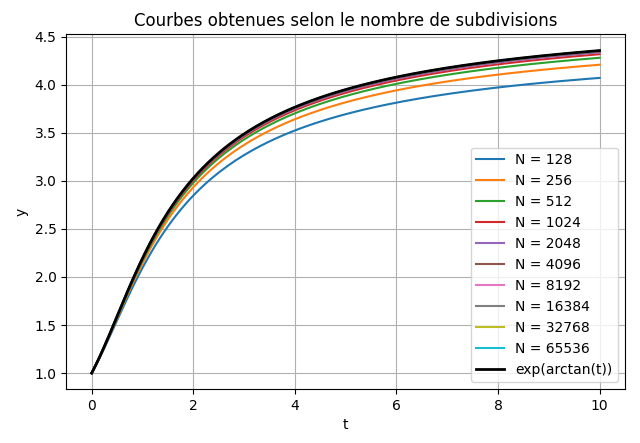
\includegraphics[width=0.45\textwidth]{res/subdivisions}
	\caption{Solutions obtenues en fonction du nombre de subdivisions, pour $y'(t) = \frac{1}{1 + t^2}$ avec $y(0) = 1$.}
	\label{fig:subdivision}
\end{figure}

Comme attendu, on observe une convergence de la solution vers la solution exacte (tracée en noir)
lorsque le nombre de subdivisions augmente.

Sur l'ensemble des méthodes de résolution étudiées, la plus précise est celle de Runge-Kutta, puisqu'elle est d'ordre $4$.
En revanche, c'est aussi la plus coûteuse en temps, puisqu'elle nécessite quatre appels à la fonction $f$ pour un unique pas de temps.
La méthode d'Euler est la moins précise (ordre $1$), mais la plus rapide, puisqu'elle ne nécessite qu'un seul appel à la fonction $f$ par pas de temps.
Les autres méthodes constituent un bon compromis entre précision et temps de calcul, puisque celle du point-milieu et de Heun sont d'ordre $2$, et nécessitent deux appels à la fonction $f$.

\subsection{Champ des tangentes}
Pour continuer, nous avons implémenté la fonction \texttt{tangent\_2D} permettant de tracer le champ des tangentes,
pour les équations différentielles de dimension $2$.

La figure~\ref{fig:tangente}, montre le champ des tangentes sur une équation différentielle
de dimension $2$, à savoir $y(t)=(y_1(t),y_2(t))$, avec $y(0)=(1,0)$ et $y'(t)=(-y_2(t),y_1(t))$.
Les résultats obtenus semblent cohérents par rapport aux résultats réels.

\begin{figure}[htbp!]
	\centering
	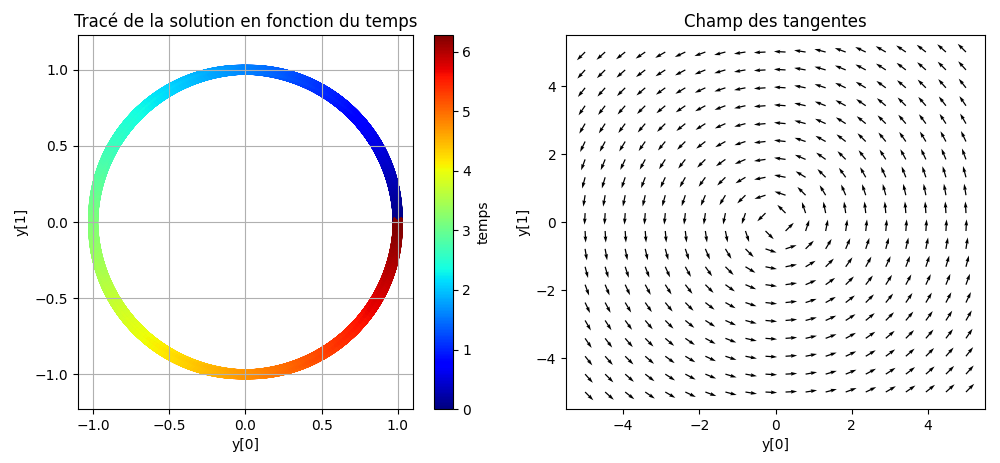
\includegraphics[width=0.7\textwidth]{res/tangente}
	\caption{Solution de l'équation différentielle, et son champ des tangentes}
	\label{fig:tangente}
\end{figure}

\vspace*{-0.7cm}
